
\documentclass[journal,UTF8]{IEEEtran}
%\usepackage{ctex}
\usepackage{color}

%
\usepackage{cite}

\ifCLASSINFOpdf
 \usepackage[pdftex]{graphicx}
  % declare the path(s) where your graphic files are
 \graphicspath{{../pdf/}{../jpeg/}}
  % and their extensions so you won't have to specify these with
  % every instance of \includegraphics
\DeclareGraphicsExtensions{.pdf,.jpeg,.png}
\else
  % or other class option (dvipsone, dvipdf, if not using dvips). graphicx
  % will default to the driver specified in the system graphics.cfg if no
  % driver is specified.
\usepackage[dvips]{graphicx}
  % declare the path(s) where your graphic files are
\graphicspath{{../eps/}}
  % and their extensions so you won't have to specify these with
  % every instance of \includegraphics
\DeclareGraphicsExtensions{.eps}
\fi

\usepackage[cmex10]{amsmath}

%\usepackage{algorithmic}
\usepackage[ruled]{algorithm2e}
\usepackage{array}

\ifCLASSOPTIONcompsoc
  \usepackage[caption=false,font=normalsize,labelfont=sf,textfont=sf]{subfig}
\else
  \usepackage[caption=false,font=footnotesize]{subfig}
\fi

\hyphenation{op-tical net-works semi-conduc-tor}



\begin{document}
%
% paper title
% can use linebreaks \\ within to get better formatting as desired
% Do not put math or special symbols in the title.
\title{A VCA Protocol Based Multi-level Flexible Architecture on Embedded PLCs for Visual Servo Control }

\maketitle

\begin{abstract}
The visual system, motion control system, and programmable logic controller ($PLC$) system are becoming increasingly inseparable and complex, however there are few works researching the integration of these three systems to ease the complexity. Most of them are focusing on their applications individually. We propose a flexible multi-level architecture which is based on a $VCA$ protocol to address the integration problem. The multi-level includes flexible layer, control layer, and algorithm layer. The flexible layer is adopted to seamlessly integrate visual system and embedded PLC ($ePLC$) system. The $VCA$ protocol is designed for data interaction between the layers. Correspondingly, a customized hardware, memory allocation, Petri-Net based multithreading structure are described to support the proposed flexible architecture. At last, we implement two cases using the proposed $VCA$ protocol based flexible architecture in which the generality of the proposed flexible architecture is verified. In first case, the winding machine with visual system implements regular winding effect by the correction of $\theta$. In the second case, the binocular catching robot uses the cameras to track the trajectory and send to $ePLC$. By adjusting the speed and position, the robot can catch the ball successfully.
\end{abstract}

% Note that keywords are not normally used for peerreview papers.
\begin{IEEEkeywords}
motion control, visual servo control, embedded PLC, multi-level architecture, Petri Net
\end{IEEEkeywords}

% For peer review papers, you can put extra information on the cover
% page as needed:
% \ifCLASSOPTIONpeerreview
% \begin{center} \bfseries EDICS Category: 3-BBND \end{center}
% \fi
%
% For peerreview papers, this IEEEtran command inserts a page break and
% creates the second title. It will be ignored for other modes.
\IEEEpeerreviewmaketitle



\section{Introduction}
Integration technologies are driving the industrial automation \cite{Kazmierkowski2007Integration}. The continuously integrations of sensors, controllers, robots, tools, etc., bring the concepts of self-aware equipment, intelligent factory, CPS, etc. \cite{Wan2018An,Chekired2018Industrial}. Recent researches \cite{Colombo2006An,Vaccaro2010An,Dean2017Integration} introduce the development of integration technologies. In industrial automation, PLC system,  motion control system, and visual system become more and more important and inseparable \cite{Feng2002Integrating,Chang2006Motion,Feng2005Practical}. In addition, the advances of edge computing, fog computing, and edge artificial intelligence \cite{Hu2017Fog,Hou2018Green,PaceAn} put forward new challenges on edge equipment of these systems.

\subsection{Motivations}
Recently, advances in image processing and pattern recognition contribute to the thriving of visual system which has been applied in various fields. By extracting features from the image, the visual system could obtain parameters to replace human visual system to address lots of tasks; specially, the ever-growing requirements in industrial scenarios; e.g., works that should be finished in dangerous environment, tasks that human vision is difficult to satisfy, or applications in some large scale industrial production that numerous visual systems are needed. 

After the visual processing, in most cases, the motion control system as the power of automation is constantly needed to drive some actuators to finished some severe tasks, which remarkably benefits the replacement of labor force. 

Furthermore, PLCs have become a base of automation owning to its high reliability and easy programming\cite{Hossain2014Advanced}. Lots of researches are focusing on it to extremely extend its applied field; for instance, \cite{Jiang2013System,Jiang2013Bayesian} guarantee the reliability by verifying the program of PLCs, \cite{Gerk2006Advanced,Dominic2016PLC} improve the performance of PLCs using advanced algorithms, \cite{wu2018customized} alleviates the development complexity of PLCs with a special software structure, \cite{Sch2013Development} pose methods to update PLC programs dynamically.


In addition, the visual system, motion control system, and PLC system are becoming increasingly inseparable. \cite{Chen2014A} is a typical case that describes how the three parts collaborate. The visual system analyzes the context and get error put into the motion control system. Simultaneously the PLC is analyzing the information, such as the position limitation of every axis, to make some logical judgments accordingly. Regarding the normal development of these applications, the three systems are developed individually and using the communication protocol combines them. However, this method should be always redesigned the programs in these systems because of the difference of visual algorithms, motion control algorithms and their organized logic programs. In addition, the logic and motion control are always mixed together to develop in motion-control-supported PLC, and there are also lots of communication protocols (e.g., EtherCat, Modbus, CAN, etc.). Considering the high requirements of today’s applications, this becomes a cumbersome task.

Hence, how to pose a flexible structure to the integration of visual system, motion control system, and PLC system which will ease the complexity and satisfy the ever-growing requirements attracts our interest.

\subsection{Related Works}

Visual control system is combined of special motion control system and visual system which has been applied in various fields, such as transport \cite{Xing2014Intersection}, circuit detection\cite{Nian2005An}, sorting system, welding\cite{Chen2014A}, assembling\cite{Wang2008Visual,Xiao2014Visual}, robot\cite{Wu2013Cloud,Tsai2017A}, unmanned aerial vehicles\cite{Guenard2010A,Serra2016Landing}, and sorting\cite{Sun2013Automatic}. These works address their problems in relevant fields. However, all these solutions are based on special motion control system and visual system.

Additionally, the integration of logic control and motion control has variously deep researches \cite{Ioannides2004Design,Shi2016The,Fang2017Design, syaichu2011model}. \cite{Ioannides2004Design,syaichu2011model} realize the motion control directly in PLC. \cite{Peng2011Linear, Qian2014A, OMRON2006CS1W} use motion control module collaborated with PLC to implement their applications. However, owing to the confusion of the development method in these works, PLCopen organization released a related standard \cite{PLCopen2005Function} which standardizes the motion control in PLC. Based on this standardization, \cite{S2006Advanced} provides an advanced implementation in distributed automation system, and companies, such as 3S \cite{3S2017Logic}, provide some tools for users. \cite{wu2018customized} also poses a customized real-time compilation method to reduce the development complexity.

Above works provide impressive integrations on visual servo control system and PLC with motion control functions, however there are few works researching the integration of visual system, motion control, and PLC. Most of applications are focusing on their applications with three individual systems, such as \cite{Chen2014A}. Hence, an integration structure of PLC system, motion control system, and visual system should be provided to reduce the complexity and expand the application fields.

\subsection{Our Contributions}
We propose a flexible multi-level architecture which is based on a $VCA$ protocol to address the problem of integration of PLC system, motion control system, and visual system. The multi-level includes flexible layer, control layer, and algorithm layer. The $VCA$ protocol is designed for data interaction between the layers. Correspondingly, customized hardware, memory allocation, and Petri-Net based multithreading structure are described to support the proposed flexible software architecture.

In the remaining paper, in Section \ref{SystemStructure}, the hardware and software structure and memory allocation are introduced. In Section \ref{Integration}, the mechanism of $VCA$ protocol is addressed in detail. In Section \ref{Execution}, we illustrate the execution process of the proposed system. Then, we implement two cases which are binocular catching robot and winding machine with visual system in Section \ref{Case}. In the last section, we conclude our works.

\section{System Architecture}
\label{SystemStructure}
\subsection{Hardware Structure}
The hardware is comprised of ePLC system ($ES$) and visual system ($VS$). The $ES$ is a customized structure. The number of digital input/output, analog input/output and controlled servo system could be increased according to requirements. Fig. \ref{fig:Hardware} shows a typical $ES$ which adopts two processor architecture. The shared memory is used to interact data between master and slave processor. The $VS$ normally contains one or more cameras, and a CPU for visual tasks. The communication between $ES$ and $VS$ could adopt multiple protocols, such as TCP, modbus, and CAN.

\begin{figure}
	\centering
	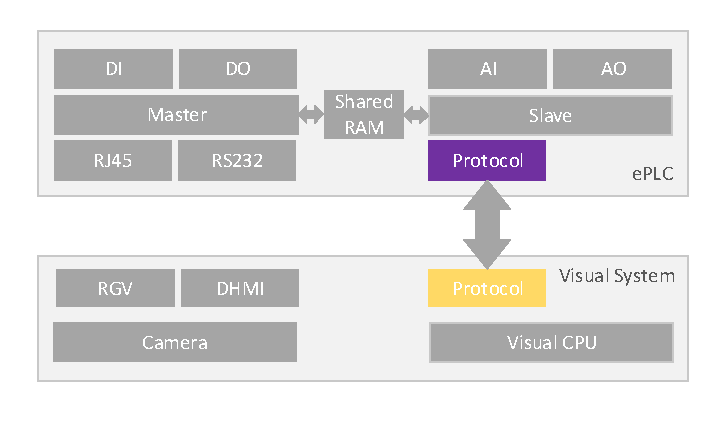
\includegraphics[width=3.5in]{fig/Hardware.pdf}
	\caption{Hardware architecture of typical $ES$ and $VS$. The $ES$ adopts two processor architecture and the $VS$ contains one camera and a CUP. The communication between $ES$ and $VS$ adopt the CAN Bus.}
	\label{fig:Hardware}
\end{figure}
\subsection{Software Structure}
The software of the proposed multi-level flexible structure is shown as in Fig. \ref{fig:Software}. To our best knowledge, the $VS$ commonly contains several visual algorithms and every algorithm could extract some required parameters form pictures or videos. Meanwhile, the $ES$ is comprised of modules which conclude logic part and algorithms. The algorithms here mainly donate motion control algorithms. The structure contains three layers: flexible layer ($FL$), control layer ($CL$), and algorithm layer ($AL$).

\textbf{Flexible layer}: these layer is responsible for joint the $VS$ and $ES$, which consists of $PLC$ interface and visual interface. The parameters are framed with $VCA$ protocol frame (henceforth, $VCA$ protocol frame is abbreviated form of $PF$) interacted between $VS$ and $ES$. Furthermore, a special protocol template ($PT$) is saved in both systems to illustrate the protocol.

\textbf{Control layer}: this is independent form algorithm layer to cope with the logic tasks. This make it possible to run the logic task and algorithm task in different processors.

\textbf{Algorithm layer}: it is mainly comprised of various types of algorithms. The independent algorithm layer makes the algorithms with high performance requirement that could be built in individual processors. 


\begin{figure}
	\centering
	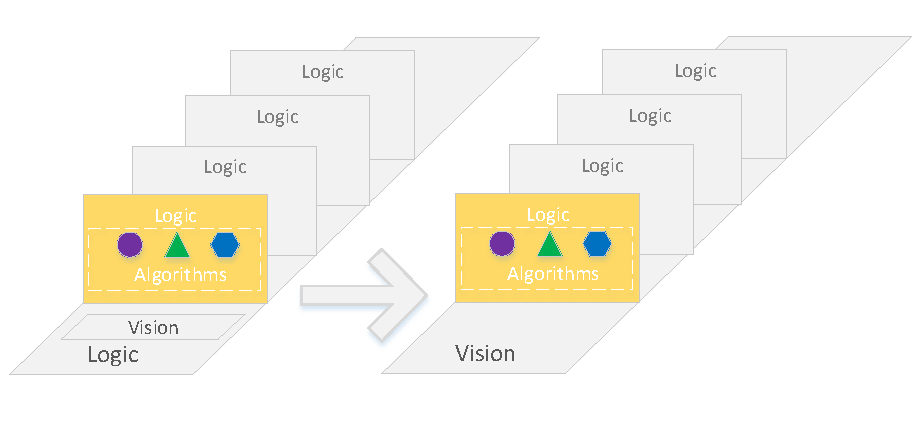
\includegraphics[width=3.5in]{fig/Software.pdf}
	\caption{Multi-level flexible architecture contains three layers: flexible layer, control layer and algorithm layer.}
	\label{fig:Software}
\end{figure}


\subsection{Memory Allocation}
\begin{figure}
	\centering
	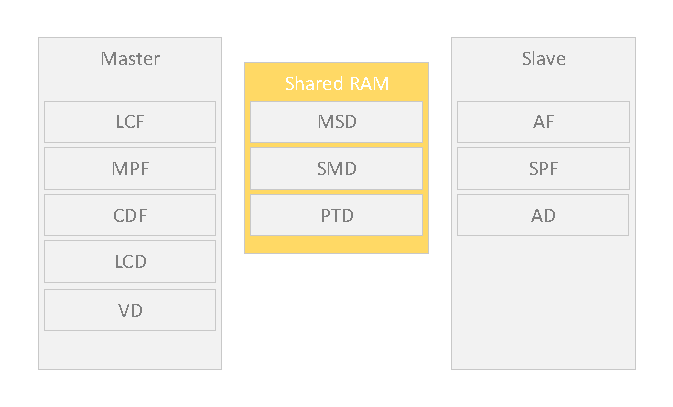
\includegraphics[width=3in]{fig/RAM.pdf}
	\caption{Memory allocation of master processor, shared ram and slave processor.}
	\label{fig:RAM}
\end{figure}
The dedicated storage area of $PLC$ in memory is made up of bit data area ($M$ area) and byte data area ($D$ area). Meanwhile, we regard $M$ area and $D$ area as set $M$ of bit and set $D$ of byte. Henceforth, if $\exists$ set $S$, we define its subscripted lowercase letter $s_i$ as an element of $S$ and the subscripted $i$ is used to distinguish the elements.Fig. \ref{fig:RAM} shows the memory allocation of master processor, shared RAM and slave processor. The shared $RAM$ is a special structure to fast data interaction between master and slave processors. In more general cases, the $MSD$ is located in master processor, the $SMD$ and $ADF$ are located in slave processor and the $PT$ is in both master and slave processors. 

In master processor, its RAM contains the special areas: 1) Module control flag area ($MCF$) are used to start the modules. 2) Master processor data interaction flag area ($MPF$) contains begin data transfer flag from master to slave ($MSB$), transfer state of master from master to slave ($MSF$), acknowledge flag of master from master to slave ($MSA$) ,and transfer state of master from slave to master ($MSS$). 3) Module data saved flag area ($MDF$) denotes whether the module data are saved. 4) Logic control data area ($LCD$) are used to store the control frame. Every element $lcd_i$ is associated with a specified module. 5) $VCA$ protocol frame data area ($VD$) stores all the frames received form the $VS$.  

In shared RAM, it could be read by both of master and slave processors and consists of the special areas: 1) Master processor data interaction data area ($MSD$) stores the data delivered from slave processors. 2) Slave processor data interaction data area ($SMD$) stores the data delivered from master processor. 3) Algorithm data saved flag area ($ADF$) denotes whether the algorithm data are saved. 4) Protocol template data area ($PTD$) stores the protocol template which contains $PT$s from $VS$ to $ES$ and from $ES$ to $VS$.


In slave processor, the RAM is comprised of the special areas: 1) Algorithm flag area ($AF$) includes algorithm flag of execution ($AFE$) and algorithm flag of state ($AFS$). 2) Slave processor data interaction flag area ($SPF$) includes the begin data transfer flag from slave to master ($SMB$), transfer state of slave from slave to master ($SMF$), acknowledge flag of slave from slave to master ($SMA$), and transfer state of slave from master to slave ($SMS$). 3) Algorithm data area ($AD$) saves data which help specified algorithm executing.

 We define the $\mathcal{I}$ to interact data between master processor and slave processor. It contains two parts: transferring data from master to slave ($\mathcal{I}_{mts}$) and transferring data from slave to master ($\mathcal{I}_{stm}$), which is defined below:
 \begin{equation}
 \left\{
 \begin{array}{l}
 \mathcal{I}_{mts} = \mathcal{L} (msb_i,msf_i,sma_i,sms_i,smd_i)\\
 \mathcal{I}_{stm} = \mathcal{L} (smb_i,smf_i,msa_i,mss_i,msd_i)
 \end{array}
 \right.
 \end{equation}
 Where $\mathcal{L}$ is the function to implement the process of data interaction between master and slave processors. $\mathcal{I}_{mts}$ and $\mathcal{I}_{mts}$ use the same function $\mathcal{L}$. The process of $\mathcal{I}_{mts}$ is described as follows: the master processor sets $msb_i$ one, sets $msf_i$ one, sends data to $smd_i$,  recovers $msb_i$ to zero, and informs slave processor to get the data; the slave processor sets $sms_i$ one, checks the data of $msd_i$, sets $sma_i$ one, feeds back the master processor to end the transferring, recovers $sms_i$ zero, and recovers $sma_i$ zero; at last, the master processor recovers $msf_i$ zero.     
 

%%%Fig.6. Distribution of dedicated public data area.
\section{Integration of $VS$ and $ES$}
\label{Integration}

\subsection{$VCA$ $PT$}
\begin{figure}
\centering
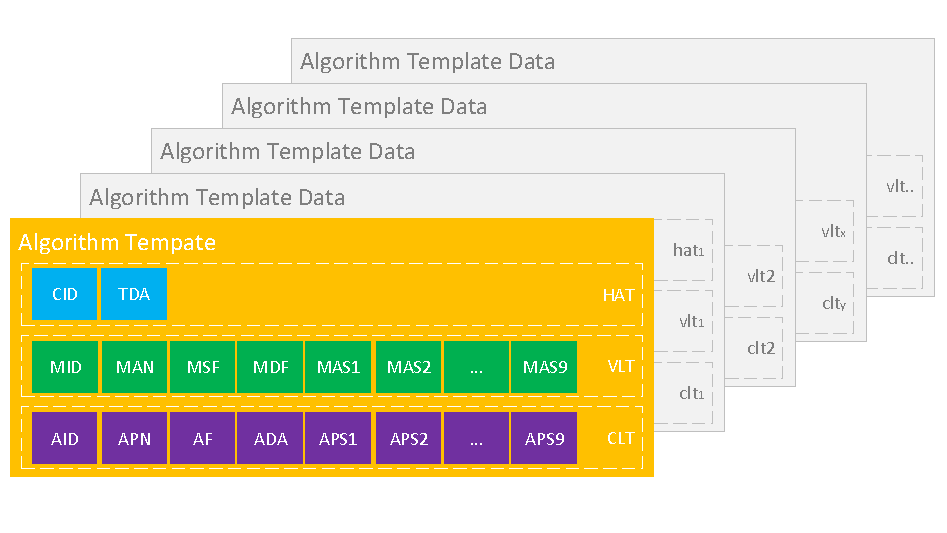
\includegraphics[width=3.5in]{fig/PT.pdf}
\caption{A $PT$ uniquely corresponds to a type of application. It contains four parts: head of protocol template, visual layer template , control layer template and algorithm layer template.}
\label{fig:PT}
\end{figure}
In cater to most applications, we propose a $VCA$ protocol based multi-level flexible architecture. As shown in Fig. \ref{fig:PT}, a protocol template ($PT$) is adopted to support various types of implementations and a $PT$ uniquely corresponds to a type of application. In the flexible architecture, users only need to redesign and reload the $PT$ and then they can reuse the visual servo system again. The $PT$ could be loaded into a stationary address of visual system and $ePLC$ system. After restarting both systems, it will be put into a fixed area of $RAM$. The parsing modules form both systems will read it when parsing the $PF$. The $VCA$ protocol could be used to bidirectionally transfer $PF$ using the same $PT$ and algorithms of framing and deframing.  
 
 The $PT$ is defined below:
  \begin{equation}
 \left\{
 \begin{array}{l}
 PT = \{HPT, VPT, APT, PPT\}\\
 HPT = \{CID, TDA\}\\
 VPT = \{MID, MAN, MDN, MDA, MSF, MDF, \\
 \qquad\qquad\quad \bigcup_{x=1}^i MAF_x, \bigcup_{x=1}^j CPS_x\}\\
 APT = \{AID, APN, ADA, AF, ADF, \bigcup_{y=1}^i APS_y\}\\
 PPT = \{PID, VID, VAR\}
 \end{array}
 \right.
 \end{equation}
 

 The $PT$ contains four parts: head of protocol template ($HPT$), VCA protocol template ($VPT$), algorithm protocol template ($APT$) and parameter protocol template ($PPT$). Every part explains as follows: 
 \begin{enumerate}
 	\item $HPT$: this part includes communication unique ID ($CID$), template data storage address ($TDA$). Every $PT$ only has one $HPT$.
 	\item $VPT$: it consists of module unique ID ($MID$), module contained algorithm number ($MAN$), , module contained data number ($MDN$), module data start address ($MDA$), module start flag ($MSF$), module data saved flag ($MDF$), module contained algorithm IDs ($MAS_x$) . $VLT$ is not $\emptyset$. Every $VPT$ includes $MAN$ algorithm IDs. 
 	\item $APT$: it is comprised of algorithm unique ID ($AID$), algorithm contained parameter number ($APN$), algorithm data start address $ADA$, algorithm data saved flag ($ADF$), algorithm contained parameter IDs ($APS_y$). $CLT$ is not $\emptyset$. Every $APT$ includes $APN$ parameter IDs.
 	\item $PPT$: it contains parameter unique ID ($PID$), its relevant visual algorithm ID ($VID$) and the conversion ratio of visual algorithm parameters and motion algorithm parameters ($VAR$).  
 \end{enumerate}
 \subsection{$VCA$ $PF$}
 The $VCA$ protocol frame ($PF$) contains parameter frames and algorithm frames in its data field and the algorithm protocol frame contains several parameter frames as shown in \ref{fig:Protocol}. 

 \begin{enumerate}
	\item $PF$: it consists items of $MID$, visual frame length ($VFL$), data from parameter frames ($PFDATA$) and data form algorithm frames($AFDATA$).The $PFDATA$ and $AFDATA$ contains several parameter frames and control frames, respectively. The $MID$s both in $PT$ and $PF$ need one-to-one correspondence.
	\item Algorithm frame: it is comprised of $AID$, control frame length ($CFL$) and $PFDATA$. The $AID$s both in algorithm frame and $PF$ need one-to-one correspondence.
	\item Parameter frame: it contains $PID$, $PDATA$. $PID$ is also the address of $PDATA$. The $PID$s both in parameter frame and $PF$ need one-to-one correspondence.
\end{enumerate}


\begin{figure}
	\centering
	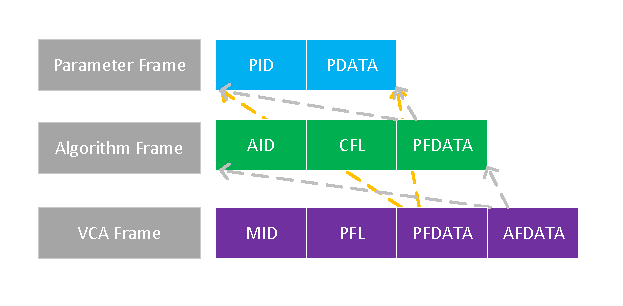
\includegraphics[width=3in]{fig/Protocol.pdf}
	\caption{ $VCA$ protocol frame contains parameter frames and algorithm frames in its data field and the algorithm protocol frame contains several parameter frames.}
	\label{fig:Protocol}
\end{figure}
\subsection{Framing of $PF$}
The framing contains three steps: $VCA$ framing, $CL$ framing, and $AL$ framing. Transfer data area ($TD$) saves the data to be transferred and it is indexed by the $PID$. In the $VS$, it represents the parameters obtained form the visual algorithms. In the $ES$, the data come from the $RAM$.   


\textbf{\emph{VCA} Framing}: the process is realized as the Algorthm \ref{alg1}. It searches the $PT$ with $mid$ to find the relevant $vlt_x$. Through it, we can obtain the $man$ and $mdn$. According to $man$ and $mdn$, the Algorithm \ref{alg3} and Algorithm \ref{alg2} are called to gain the $pfdata$ and $afdata$. Then, it is finished after calculating the length ($vfl$).

\textbf{\emph{CL} Framing}: Algorthm \ref{alg2} illustrates the process. It seeks the $PT$ to gain the $alt_y$ which contains the $apn$. According to $apn$, call the Algorithm \ref{alg3} to obtain the $pfdata$ and then calculate the length ($cfl$) to finish the $AL$ framing.  

\textbf{\emph{P} Framing}: Algorthm \ref{alg3} shows the process. The $VS$ obtains the $alt_z$ from $FT$ and then combines the $pid$ and $pdata$.


\begin{algorithm}
	\label{alg1}
	\caption{$VCAFraming$}%算法名字
	%\LinesNumbered %要求显示行号
	\KwIn{$mid$, $TD$}%输入参数
	\KwOut{$PF$}%输出
	SearchPT ($mid$, $vpt_x$)\;
	$PF.mid\leftarrow mid$\; 
	\For{$i=0$;$i<vpt_x.mdn$;$i++$}{
		ALFraming ($vpt_x$.$cps$[i], $TD$,$pfdata$)\;
	}
	\For{$i=0$;$i<vpt_x.man$;$i++$}{
		CLFraming ($vpt_x$.$mas$[i], $TD$,$afdata$)\;
	}
    $PF.pfdata\leftarrow$ $pfdata$\; 
    $PF.afdata\leftarrow$ $afdata$\; 
	$PF.vfl\leftarrow$ ($vpt_x.mdn+vpt_x.man$) $\times$ 4 + 8\;
\end{algorithm}

\begin{algorithm}
	\label{alg2}
	\caption{$CLFraming$}%算法名字
	%\LinesNumbered %要求显示行号
	\KwIn{$aid$, $TD$, $afdata$}%输入参数
	\KwOut{$afdata$}%输出
	SearchPT ($aid$, $apt_y$)\;
	Create $clf$\;
	$af.aid\leftarrow$ $aid$\;
	\For{$i=0$;$i<apt_y.apn$;$i++$}{
		ALFraming($apt_y$.$aps$[i], $TD$, $pfdata$)\;
	}
	$af.cfl \leftarrow$ $apt_y.apn \times 4$ + 8\;
	$af.pfdata \leftarrow$ $pfdata$\;	
	$afdata\leftarrow$ $afdata$ + $clf$\;	 
\end{algorithm}
\begin{algorithm}
	\label{alg3}
	\caption{$ALFraming$}%算法名字
	%\LinesNumbered %要求显示行号
	\KwIn{$pid$, $TD$,$pfdata$}%输入参数
	\KwOut{$pfdata$}%输出
	SearchPT ($pid$, $ppt_z$)\;
	Create $pf$\;
	$pf.pid\leftarrow$ $pid$\; %How to address the problem of id is same with address.
	$pf.pdata \leftarrow$ $TD[pid]\times ppt_z.var$\;
	$pfdata\leftarrow$ $pfdata$ + $alf$\;	 
\end{algorithm}

\subsection{Deframing of $PF$}
 The process of deframing of $PF$ divided into $VCA$ deframing, $CL$ deframing, and $AL$ deframing. Received Data ($RD$) area are used to save the deframing parameters. the $RD1$, $RD2$ and $RD3$ are different temporarily data stored area. In the $VS$, $RD3$ are the data fed back to visual algorithms. In the $ES$, the $RD1$, $RD2$ and $RD3$ donate $LCD$, $MSD$ and $AD$, respectively.

\textbf{\emph{VCA} deframing}: As illustrated in Algorithm \ref{alg4}, obtain the $mid$ and $pfl$ form the start four and following four bytes data of $PDF$, respectively. Search the $PT$ to gain the relevant $vpt_x$. Send the $pfl-8$ bytes start form the eighth byte of $PDF+8$ to the address $mda$ of $vlt_x$.

\textbf{\emph{CL} deframing}: According to $mid$, search $PT$ to find the relevant $vpt_x$. Loop deal with the $mda$ times of the parameter frame. In each loop, the data are sent to $RD3$ with the relevant $pid$. Loop deal with the $man$ times of the algorithm frame. In each loop, use the $aid$ to find $apt_y$ and then send the $afdata$ to correlative address of $RD2$. Algorithm \ref{alg5} is described the process.

\textbf{\emph{AL} deframing}: Use $aid$ to get its $apt_y$. Loop cope with the algorithm frame $apn$ times. Send the parameters to $RD3$ with the correlative $pid$. The process is shown in Algorithm \ref{alg6}.

\begin{figure}
	\centering
	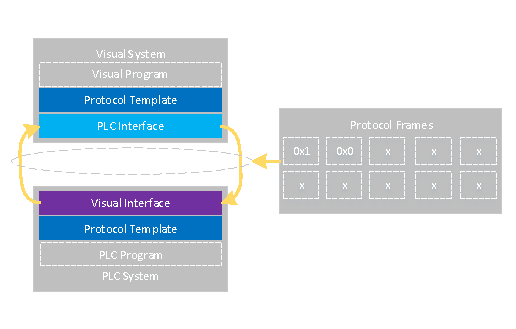
\includegraphics[width=3in]{fig/FlexibleLayer.pdf}
	\caption{ $PF$ interaction between PLC interface and visual interface.}
	\label{fig:FlexibleLayer}
\end{figure}
\begin{algorithm}
	\label{alg4}
	\caption{$VLDeframing$}%算法名字
	%\LinesNumbered %要求显示行号
	\KwIn{$PDF$}%输入参数
    $mid \leftarrow$ four bytes form $PDF$\;
    searchPT ($mid$, $vpt_x$)\;
    $pfl \leftarrow$ four bytes form $PDF+4$\; 
    $RD1[vpt_x.mda]\leftarrow$ $pfl-8$ bytes form $PDF+8$\;     	
	$PDF\leftarrow$ $PDF+pfl$\;
	value of $vpt_x.mdf\leftarrow 1$\;
\end{algorithm}

\begin{algorithm}
	\label{alg5}
	\caption{$CLDeframing$}%算法名字
	%\LinesNumbered %要求显示行号
	\KwIn{$mid$}%输入参数
	searchPT($mid$, $vpt_x$)\;
	$mda\leftarrow$ $vpt_x.mda$\;	
	\For{$i=0$;$i<vpt_x.mdn$;$i++$}{
		$RD3[RD1[mda]]\leftarrow$ 4 bytes form $mda+4$\;
		$mda\leftarrow mda+8$\;
	}
	\For{$i=0$;$i<vpt_x.man$;$i++$}{
		searchPT($vpt_x.mas[i]$, $apt_y$)\;
		$cfl\leftarrow$ 4 bytes form $mda+4$\;
		$RD2[apt_y.apa]\leftarrow$ $cfl - 8$ bytes form $mda+8$\; 
        $mda\leftarrow$ $mda+cfl$\;
        value of $apt_y.adf\leftarrow$ 1\; 
	}
\end{algorithm}

\begin{algorithm}
	\label{alg6}
	\caption{$ALDeframing$}%算法名字
	%\LinesNumbered %要求显示行号
	\KwIn{$aid$}%输入参数
	searchPT($aid$, $apt_y$)\;
	$ada\leftarrow$ $apt_y.ada$\;
	\For{$i=0$;$i<apt_y.apn$;$i++$}{
		$RD3[RD2[ada]]\leftarrow$ 4 bytes form $ada+4$\;
		$ada\leftarrow ada+8$\;
	}
\end{algorithm}


\section{System Operation Mechanism}
\label{Execution}
\subsection{Implementation of Flexible Program and Execution}
The $FL$ contains PLC interface and visual interface, shown in Fig. \ref{fig:FlexibleLayer}. They interact with each other using the agreed communication protocol which is defined as $CID$ in $HPT$ of $PT$. 

In the $ES$, the visual interface includes the following parts.

\textbf{V1}: communicates with $VS$, according to the $CID$ in $HPT$. It has three transitions. \textbf(V1.1) donates no communication and other operations; \textbf(V1.2) donates receiving $PF$s from $VS$, and \textbf{V1.3} donates sending $PF$s to $VS$. In $V1.3$, the $PF$s will be saved in the $VD$ of $ES$ and there are two pointers: $PDF$ and $PSP$, shown in Fig. \ref{fig:VisualInterface}. $PDF$ points to the address of deframing $PF$ and $PSP$ points to the address of saving $PF$. After saved the $PF$, the $PSP$ will point to the next new address according the $vfl$ of $PF$. In $V1.3$, visual interface frames $TD$ into $PF$ with the Algorithm \ref{alg1}, \ref{alg2} and \ref{alg3}. Here, the $TD$ is in $RAM$ of $ePLC$.

\textbf{V2}: Algorithm \ref{alg4} will be called. The $PDF$ will point to the next $PF$, if a $PF$ is deframed.


In the $VS$, there are following parts.  

\textbf{V1}: visual algorithms extracts the useful data and stores into array of data required to be transfered ($TD$) in which the parameters could be indexed by the $PID$.

\textbf{V2}: communicates with $ES$. It also contains three transitions. \textbf{V2.1} is no communication and other operations; \textbf{V2.1} frames $TD$ into $PF$s with the Algorithm \ref{alg1}, \ref{alg2}, and \ref{alg3} and sends the $PF$s to $ES$. Here, the $TD$ is an array in $VS$; \textbf{V2.3} receives the $PF$s form $ES$ and deframes the $PF$s with the Algorithm \ref{alg4}, \ref{alg5}, and \ref{alg6}.

\begin{figure}
	\centering
	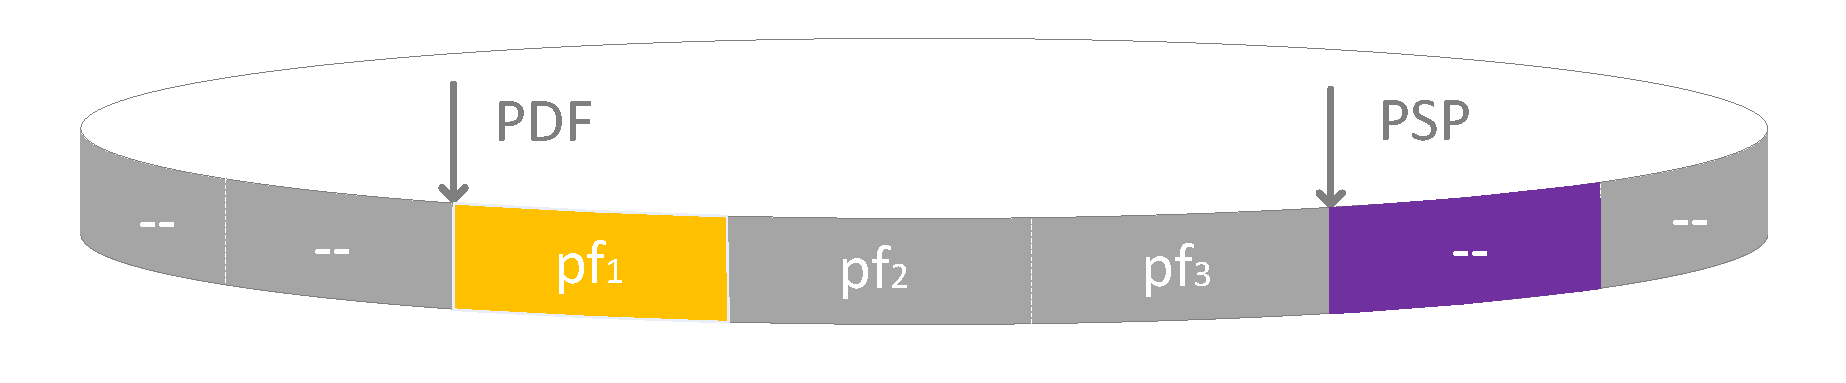
\includegraphics[width=3in]{fig/VisualInterface.pdf}
	\caption{ $PDF$ and $PSP$. $PDF$ points to the address of deframing $PF$ and $PSP$ points to the address of saving $PF$. The $PDF$ will point to the next address of $PF$ if a $PF$ is deframed. After saved the $PF$, the $PSP$ will point to the next new address according the $vfl$ of $PF$.}
	\label{fig:VisualInterface}
\end{figure}



\subsection{Implementation of Control Program and Execution}
Control program ($CP$) is responsible for organizing the modules, executing the logic program, deframing the $PF$ and interacting the data with algorithm program. The implementation of control program is described below.

\textbf{C1}: traverse the $MCF$ and $MDF$. Its contains three transitions. \textbf{C1.1} donates that every $mcf\in MCF$ and $mdf \in MDF$ is recovered to zero. \textbf{C1.2} means that both $mcf_i$ and $mdf_i$ are checked one. \textbf{C1.3} means that $mcf_i$ are checked one while $mdf_i$ is zero.

\textbf{C2}: executes Algorithm \ref{alg5}. 

\textbf{C3}: executes logic program and checks whether there is any data required to transfer.  

\textbf{C4}: the $\mathcal{P}_{mts}$ is used to send data and inform the slave processor to receive parameters and start algorithms.   

\textbf{C5}: checks the end of this module. $C5.1$ donates that this module executes one time. $C5.2$ donates that the logic program still requires to run.  

\subsection{Implementation and Execution of Algorithm Program }
The algorithm program ($AP$) is in $EL$. $AP=\{\mathcal{P}_{stm}, AS, ALDP\}$, where $\mathcal{P}_{stm}$ feeds back data to master processor, $AS$ contains all algorithms and $ALDP$ deframe the $AL$ frame. The execution of algorithm program is introduced below.

\textbf{A1}: traverse the $AFS$, $ADF$, and $SMB$. $A1.1$ is no program required to execute. $A1.2$ donates that $PF$s needed to be deframed is checked. $A1.3$ donates that data needed to feed back to master processor. $A1.4$ donates that a algorithm needed to be executed is checked. $A1.5$ donates that parameters of a algorithm needed to be updated is checked.  

\textbf{A2}: $ALDP$ is executed to call Algorithm \ref{alg5}. 

\textbf{A3}: the $\mathcal{P}_{stm}$ is used to feed back data to the master processor. 

\textbf{A4}: starts a algorithm.

\textbf{A5}: executes the algorithm until the end. 

\subsection{Petri-Net Based Execution of Threads}
We adopt the analogous thread structure in \cite{wu2018customized}. Three special threads are illustrated as follows: 1) visual thread is responsible for interaction with $VS$ and drives the flexible layer; 2) control thread is mainly responsible for organizing the whole program and drives the control layer; 3) algorithm thread is used to drive the algorithm layer.

\begin{figure}
	\centering
	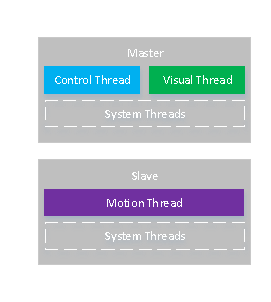
\includegraphics[width=3in]{fig/Threads.pdf}
	\caption{ Thread structure with three special threads: visual thread, Control thread, algorithm thread.}
	\label{fig:Threads}
\end{figure}

  In our works, Petri Net is adopted to describe the execution of the three threads. Every thread is a Petri-Net. We define the Petri Net as three tuple:
 
 \begin{equation}
PN = \{P,T,F\},
 \end{equation} 
 where $P$ is the finite set of places, $T$ is the finite set of transitions, and $F$ is the set of arcs. Here, $F \subset P\times T \cup T\times P$ which donates that the arcs contain form $P$ to $T$ and from $T$ to $P$.
 
 Then, we can define the execution of threads ($ET$) as follows.
 \begin{equation}
ET = \{PN_V,PN_C,PN_A\},
\end{equation} 
where $PN_V,PN_C,PN_A$ are the Petri Net of visual thread, control thread, and algorithm thread, respectively.

The $PN_V$ is donated as follows:
 \begin{equation}
\left\{
\begin{array}{l}
PN_V= \{P_V,T_V,F_V\},\\
P_V=\{P_{V1}, P_{V2}, P_{V3}\},\\
T_V=\{V_1,V_2\},\\
\end{array}
\right.
\end{equation} 
where $P_{V1}$ is idle; $P_{V2}$ is $PDF != PSP$; $P_{V3}$ is that a relevant $mdf$ is set.

The $PN_C$ is donated as follows:
\begin{equation}
\left\{
\begin{array}{l}
PN_C= \{P_C,T_C,F_C\},\\
P_C=\{P_{C1}, P_{C2}, P_{C3}, P_{C4}, P_{C5}, P_{C6}\},\\
T_C=\{C_1,C_2,C_3,C_4,C_5\},\\
\end{array}
\right.
\end{equation} 
where $P_{C1}$ is idle; $P_{C2}$ donates that a model is started and the $mdf_i$ is one; $P_{C3}$ donates that a model is started and $mdf_i$ is zero; $P_{C4}$ donates that any $msb_i$ is one; $P_{C5}$ means the end of the data interaction in which the  correlative $msf$ is zero; $P_{C6}$ donates that a module finishes one time execution.

The $PN_V$ is illustrated as follows:
\begin{equation}
\left\{
\begin{array}{l}
PN_A= \{P_A,T_A,F_A\},\\
P_A=\{P_{A1}, P_{A2}, P_{A3}, P_{A4}, P_{A5}, P_{A6}, P_{A7}, P_{A8}\},\\
T_A=\{A_1,A_2,A_3,A_4,A_5\},\\
\end{array}
\right.
\end{equation} 
where $P_{A1}$ is idle; $P_{A2}$ donates that an $adf_i$ is one; $P_{A3}$ donates that any $adf_i$ is zero; $P_{A4}$ donates that an $smb_i$ is one; $P_{A5}$ is that any $smf_i$ is zero; $P_{A6}$ is that an $afe_i$ is one; $P_{A7}$ is that an $afs_i$ is one; $P_{A8}$ is that any $afe_i$ is zero.   

The $ET$ is described in Fig. \ref{fig:threadExecution}. In the Petri Net of visual thread, if $V1.2$ executes and receives a $PF$ from $VS$, it transits from the initial position of $P_{V1}$ to $P_{v2}$. After finished deframing of a $PF$, the state transits to $P_{V3}$ and then visual thread back to execute $V1$. If there is any $FS$ which should be sent to $VS$, it will execute $V1.2$. Apart from that, ie will execute $V1.1$ and back to the position of $P_{V1}$.

In the Petri Net of control thread, the control thread executes the $C1$. The difference between $P_{C1.2}$ and $P_{C1.3}$ is that after $P_{1.2}$, the control thread transits to $P_{C2}$ and executes $C2$. Except that, it will back to $P_{C1}$. Then, the control thread runs into a module and $C3$ is run. If find any data needed to transfer to slave processor, it transits to $P_{C4}$ and executes $C4$. When finish transfer, it transits to $P_{C5}$. After execution of $C5$, according to $C5.1$ and $C5.2$, control thread transits to $P_{C3}$ and $P_{C6}$. The previous one is executed owing to that the logic program of this module is not finished.

In the Petri Net of algorithm thread, the $A1$ is executed; if any $AF$ needed to deframe, algorithm thread transits to $P_{A2}$ and after the execution of $A2$, it transits to $P_{A2}$; if any data required to feed back to master processor, algorithm thread transits to $P_{A4}$, then transfers the data, and transits to $P_{A5}$; if any algorithm should be started, algorithm thread transits to $P_{A6}$, executes the $A4$, transits to $P_{A7}$, executes $A5$ to update the parameters, and then transits to $P_{A8}$; if there are algorithms running and needed to updates parameters, algorithm thread transits to $P_{A7}$ directly and after the execution of $A5$ transits to $P_{A8}$; and above-mentioned transitions of $V1$ are executed in sequence.               

\begin{figure}
	\centering
	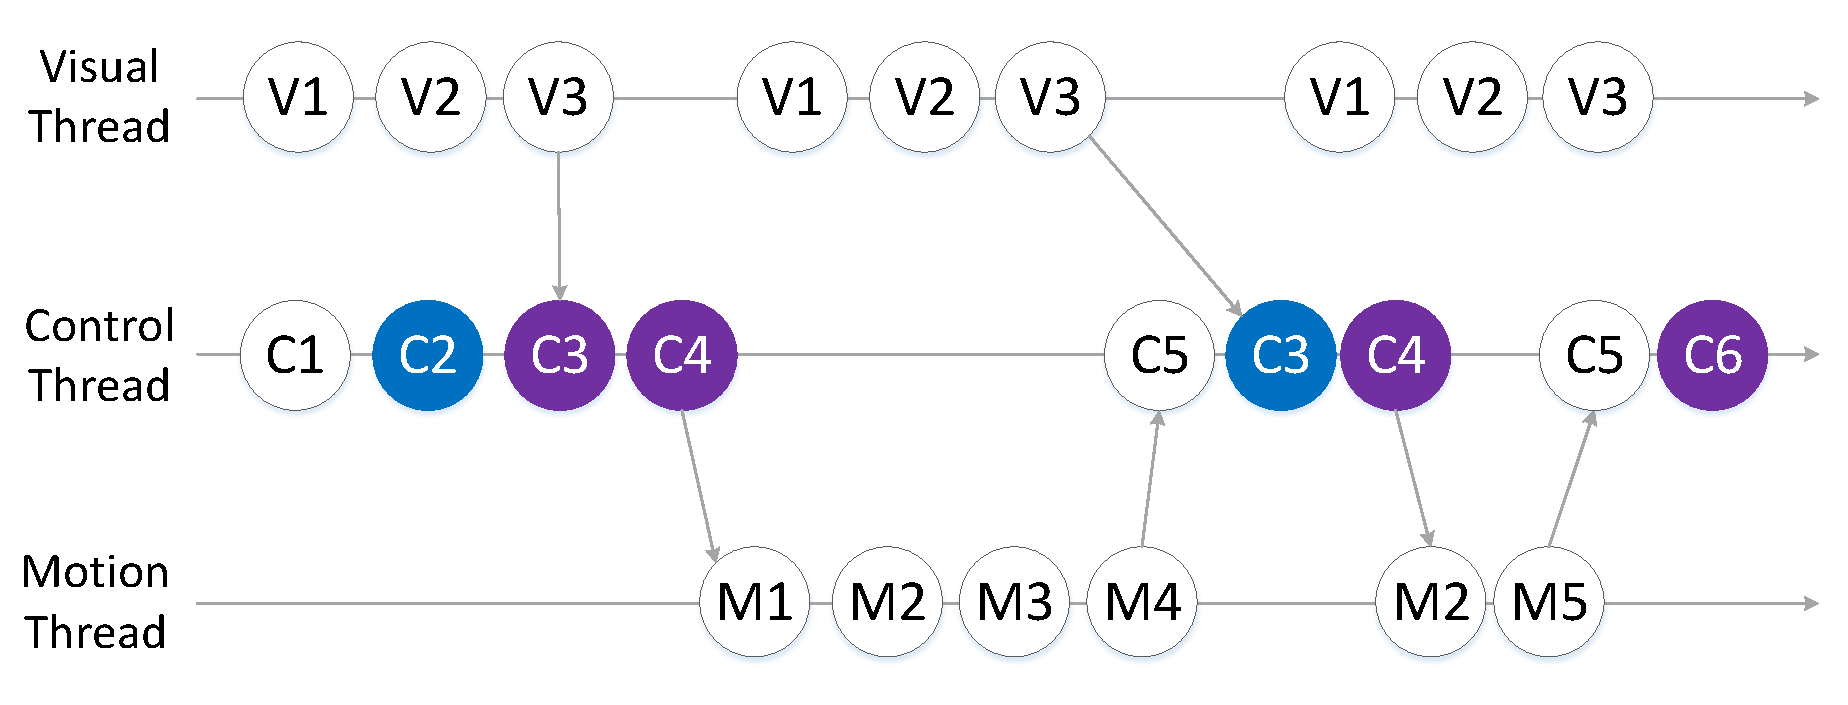
\includegraphics[width=3.5in]{fig/ThreadExecution.pdf}
	\caption{ Process of $ET$ and it contains Petri Nets of visual thread, control thread, and algorithm thread.}
	\label{fig:threadExecution}
\end{figure}

\section{Case Analysis}
\label{Case}
In this section, we introduce two scenarios of the proposed $VCA$ protocol based integration method in ePLC. With the $VCA$ protocol, users only need to code additional algorithms and change the $PT$ when the scenario of visual servo system is changed. 

\subsection{Case 1: Winding Machine with Visual System}
  
As shown in Fig. \ref{fig:Winding}, (a) is the visual system, whose CUP is ARM9 based S3C2440 and which uses the CANIF interface to communicate with OV9650 CMOS Camera; (b) is the $ePLC$, CASS-PLCA149B; (c) is the winding machine with visual system which contains two axes: the U-axis and Q-axis; (d) is shown the Winding effect, the angle of the wire, Q-axis and U-axis. In winding process, the tension of the copper wire will change irregularly, especially for the thick ones. However, we use the same speed ratio of U-axis and Q-axis which always leads to irregularity of each layer of the coil. Hence, we can use the visual system to decrease or increase the speed of Q-axis to control the angle of wire. 

Figure \ref{fig:WindingSystem} is the structure of the winding machine system. The ePLC has two chips: a master chip and a slave chip. It uses the RS232 to receive $PF$s and could control six servo systems at most. The winding machine has two axes: the U-axis and Q-axis. The $VS$ use the CMOS camera to gain winding images and transfer the digital information to ARM CUP. The ARM CUP will extract parameters from the digital information, frame $PF$s and transfer $PF$s to $ePLC$ continuously. 


\subsubsection{Design of $PT$}
In \cite{wu2018customized}, we propose the customized winding machine language which only contains 13 instructions. Here, we can use the second and third instructions to control U-axis and Q-axis, respectively. In the algorithm layer, both of them use the same motion control algorithm which controls one axis with speed and position. The process of winding is mainly to control the speed ratio of U-axis and Q-axis, hence we use the $VS$ to influence the speed of Q-axis only. The $PT$ of winding machine is illustrated in Table \ref{table:PTofWinding} in which the $pid_1$ is the speed of Q-axis and the 1000 of $var_1$ is used to multiply by the $\theta$.
\begin{table}
	\scriptsize \caption{$PT$ of winding machine}
	\label{table:PTofWinding}
	\begin{center}
		\renewcommand{\arraystretch}{1.4}
		\setlength\tabcolsep{3pt}
		\begin{tabular}{|p{1cm}|p{1cm}|p{1cm}|p{1cm}|p{1cm}|p{1cm}|p{1cm}|}
			\hline
			$cid_1$  & $tda_1$   &xxx &xxx& xxx  &xxx &xxx \\
			\hline
			0x01&0x00&& &&&\\
			\hline
			$mid_1$   & $man_1$ &$mdn_1$ &$mda_1$&$msf_1$& $mdf_1$  & $mas_1$\\
			\hline
			0x01      & 1     &   0    &0X200   &0X400   & 0X600  &0x01 \\
			\hline
			$aid_1$  & $apn_1$& $af_1$ &$ada_1$ &$aps1_1$  &xxx&xxx\\
			\hline
			0x01     & 0X1    & 0X14A  &0x1F4000 &0X0   & &\\
			\hline
			$pid_1$  &$vid_1$ &$var_1$ &xxx      &xxx   &xxx &xxx\\
            \hline
			0X0      & 0X1    & 1000   &         &   & &\\
	    	\hline
		\end{tabular}
	\end{center}
\end{table}
\subsubsection{Process of $PF$}
Table \ref{table:PFofWinding} is shown the interacted $PF$ between the $VS$ and $ES$. At first, the $VS$ detects that the $\theta$ is 2 degrees. Then, it sends the $PF$ to inform the $ES$ to increase the Q-axis speed of 2000 pulses per millisecond (p/ms). When the $\theta$ decreases to 1 degree, the increment of the Q-axis speed is changed to 1000 p/ms. Since the $\theta$ has recovered to 0, the $ES$ is informed to recover the initial speed if the Q-axis.  
\begin{table}
	\scriptsize \caption{$PF$ of winding machine}
	\label{table:PFofWinding}
	\begin{center}
		\renewcommand{\arraystretch}{1.4}
		\setlength\tabcolsep{3pt}
		\begin{tabular}{|p{1.2cm}|p{1.2cm}|p{1.2cm}|p{1.2cm}|p{1.2cm}|p{1cm}|}
			\hline
			$mid_1$   & $pfl_1$ &$aid_1$ & $cfl_1$  & $pid_1$  &$pdata_1$   \\
			\hline
			0x01    & 0x14  &0x01  &0xE     &0x01   &0x400   \\
			\hline
			0x01    & 0x14  &0x01  &0xE     &0x01   &0x200   \\
			\hline
			0x01    & 0x14  &0x01  &0xE     &0x01   &0x000   \\
			\hline
		\end{tabular}
	\end{center}
\end{table}
\begin{figure}
	\centering
	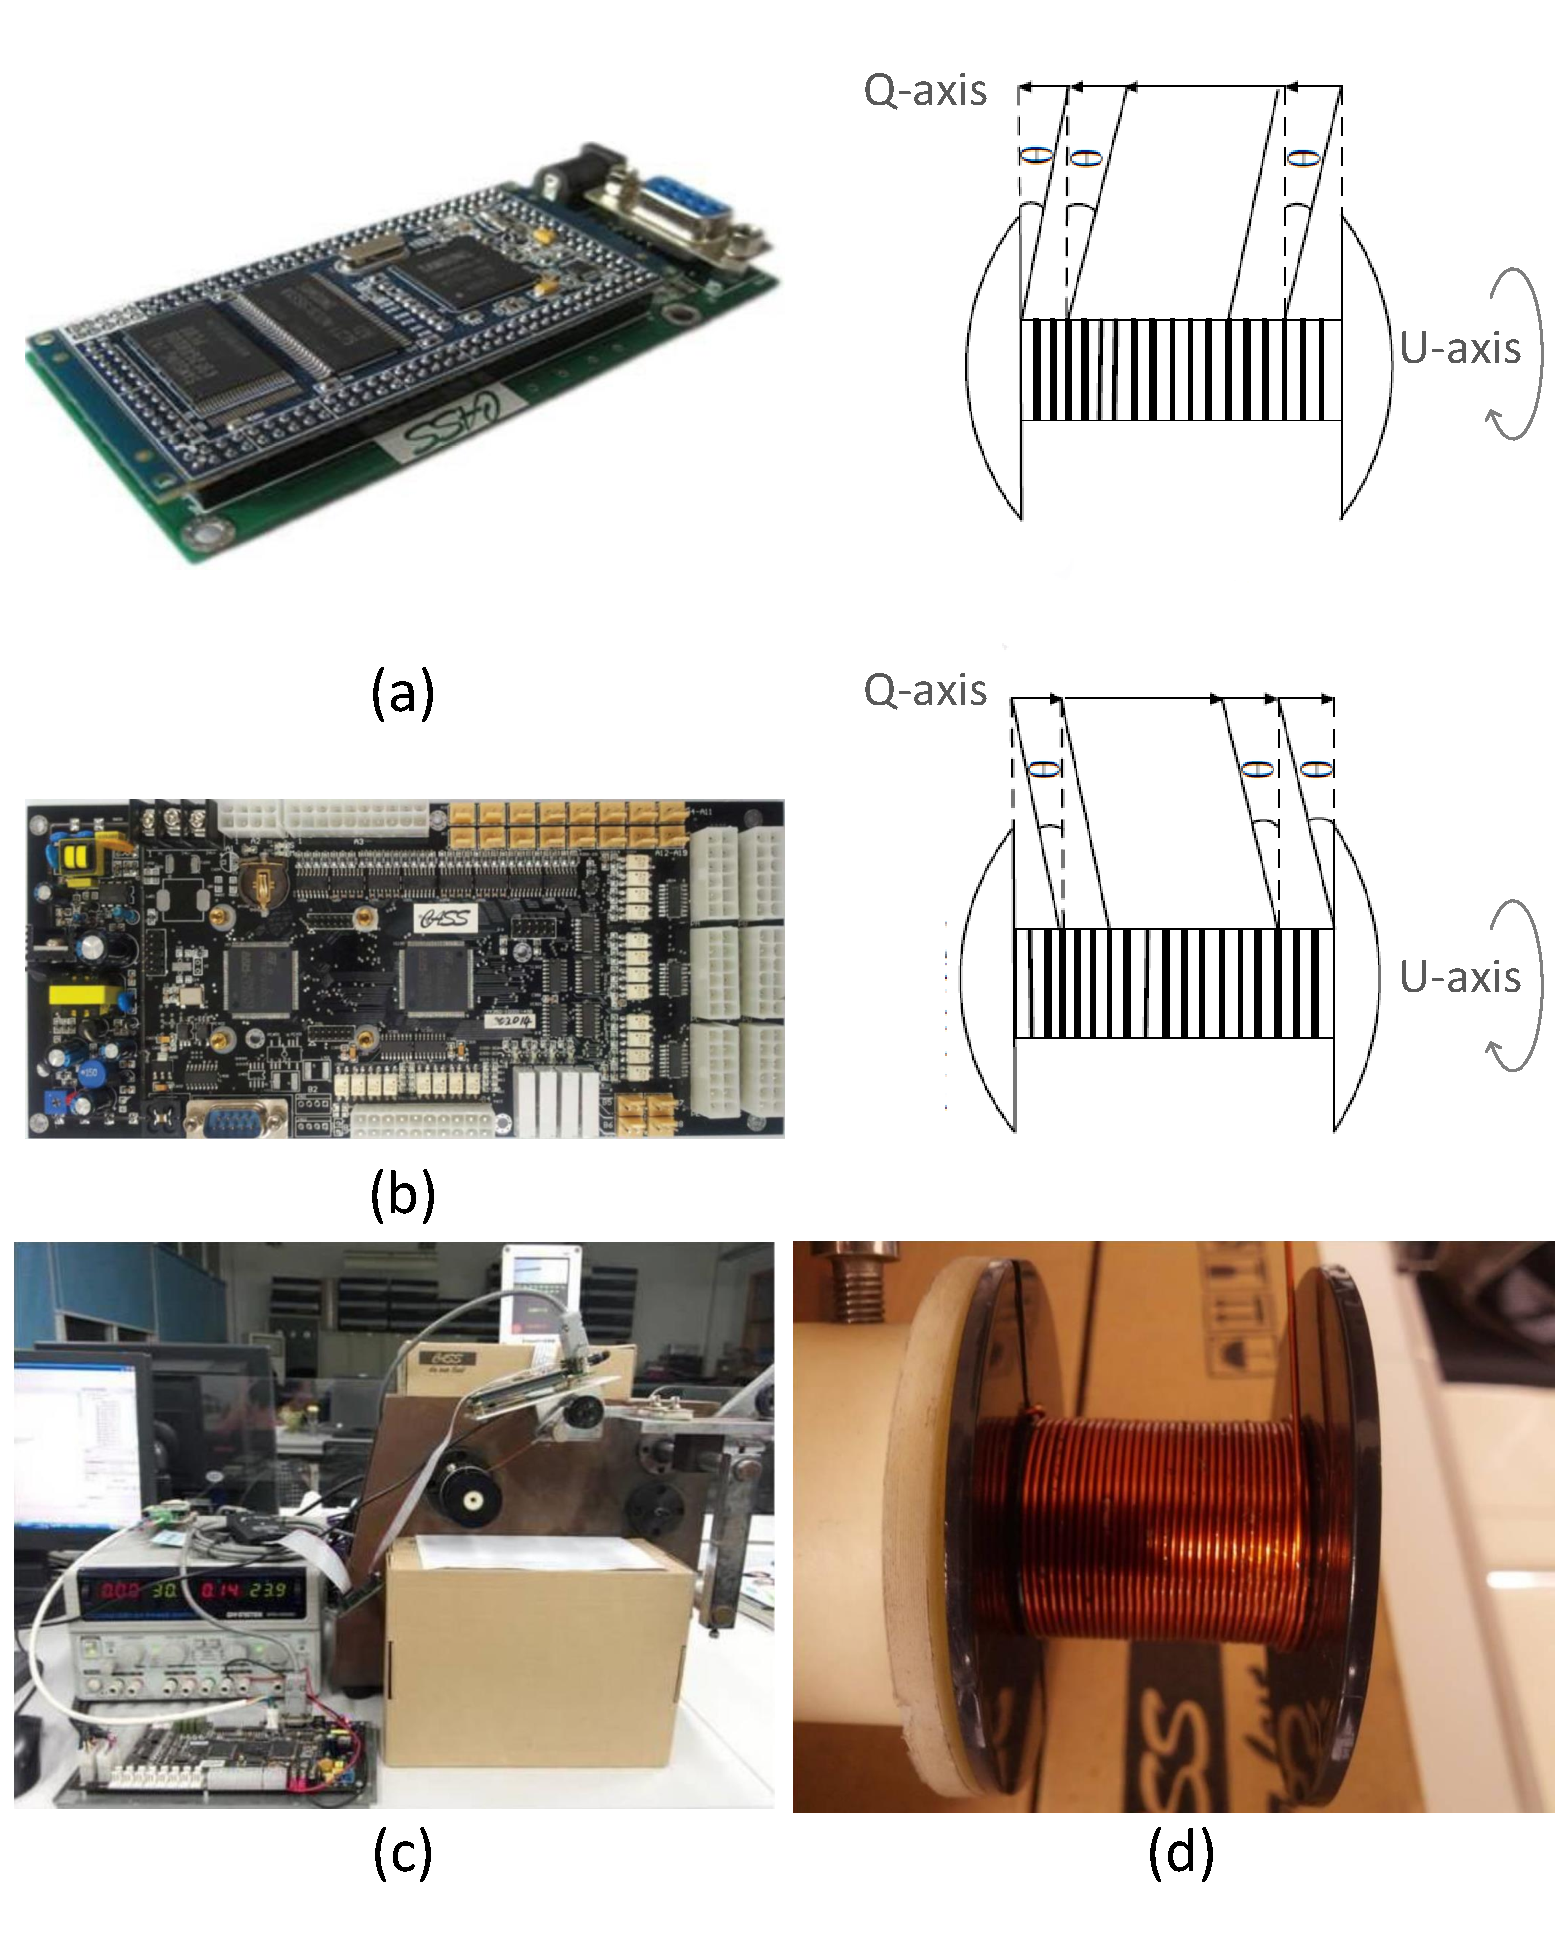
\includegraphics[width=3in]{fig/Winding.pdf}
	\caption{ (a) is the visual system, whose CUP is ARM9 based S3C2440 and which uses the CANIF interface to communicate with OV9650 CMOS Camera; (b) is the $ePLC$, CASS-PLCA149B; (c) is the winding machine with visual system which contains two axes: the U-axis and Q-axis; (d) is shown the Winding effect, the angle of the wire, Q-axis and U-axis.}
	\label{fig:Winding}
\end{figure}
\begin{figure}
	\centering
	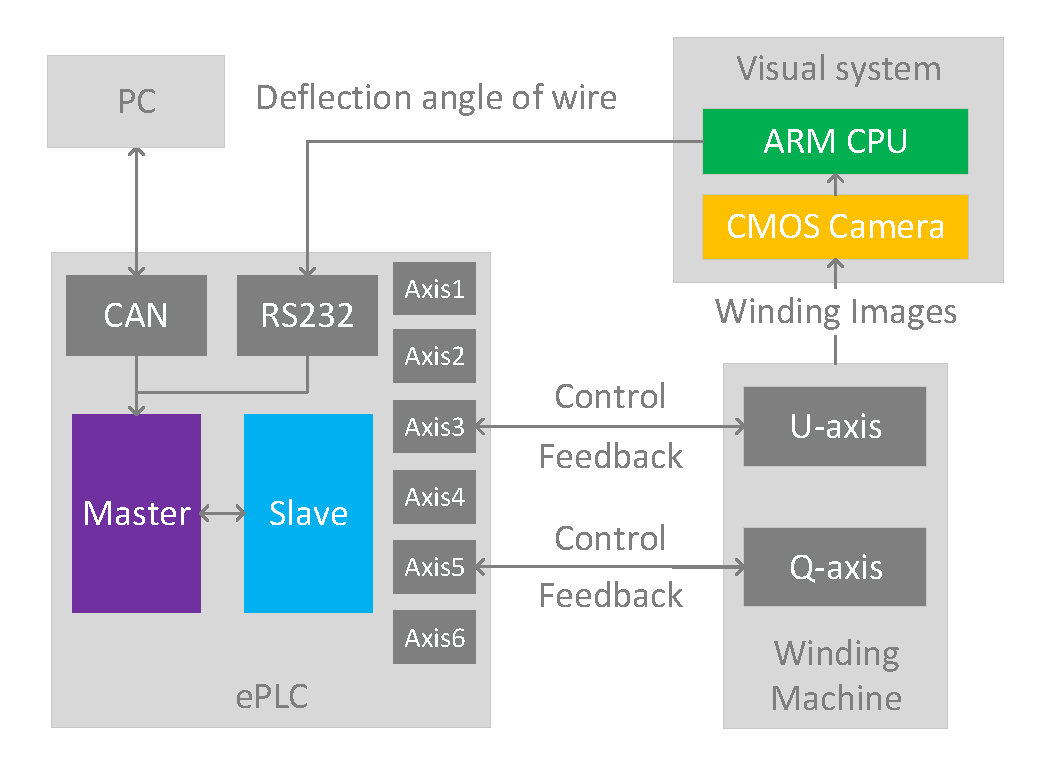
\includegraphics[width=3in]{fig/WindingSystem.pdf}
	\caption{ Structure of the winding machine system. The ePLC has two chips: a master chip and a slave chip. It uses the RS232 to receive $PF$s and could control six servo systems at most. The winding machine has two axes: the U-axis and Q-axis. The $VS$ use the CMOS camera to gain winding images and transfer the digital information to ARM CUP. The ARM CUP will extract parameters, frame $PF$s and transfer them to $ePLC$ continuously.}
	\label{fig:WindingSystem}
\end{figure}
\subsection{Case 2: Binocular Catching Robot}
\begin{figure}
	\centering
	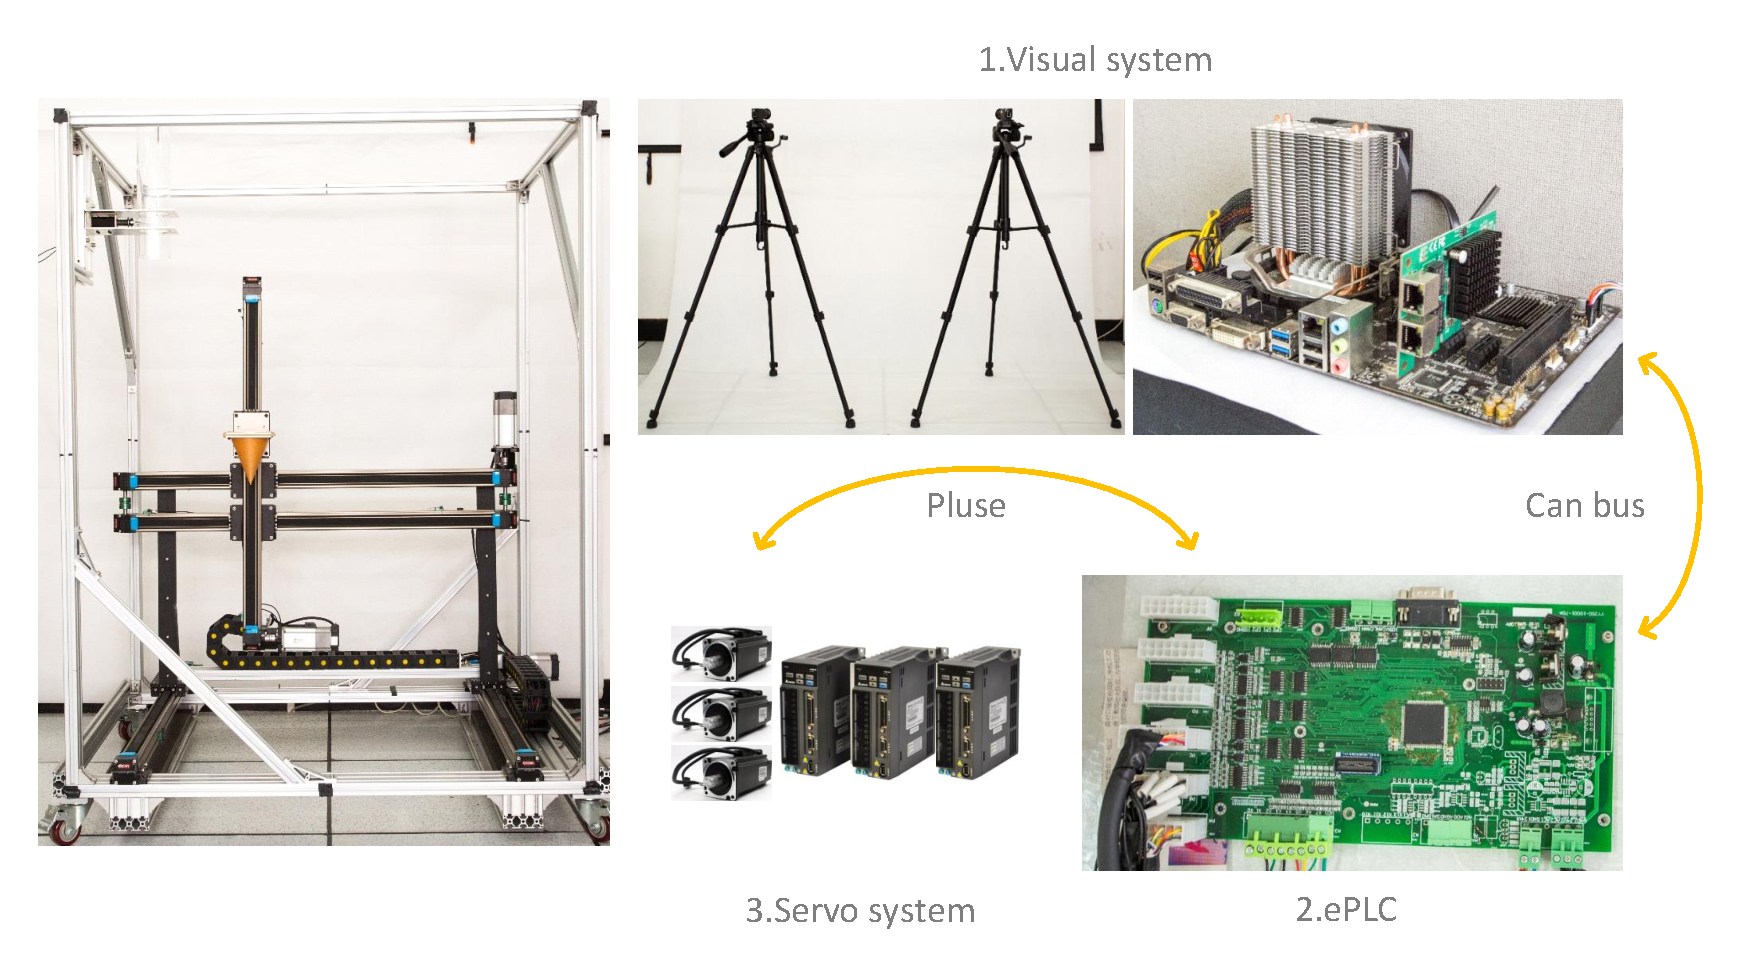
\includegraphics[width=3.7in]{fig/robot.pdf}
	\caption{ Binocular Catching Robot consists of visual system, $ePLC$ and servo system.}
	\label{fig:robot}
\end{figure}
As shown in Fig. \ref{fig:robot}, the binocular catching robot adopts two cameras to judge the position of the ball in the space. Through sending the continuously parameters to $ePLC$, the robot runs to the position to catch the ball. Finally, the robot will catch the ball. The cameras is xxx, the visual system is xxx. $ePLC$ uses the TI F28M35 chip with two cores: ARM Cortex M3 and TI C28x, which contains a shared RAM. The servo system is adopted ASDA-B2. 
\subsubsection{Design of $PT$}
The $ePLC$ is designed to control six axes parallel. We adopt the same algorithm of Q-axis and U-axis in case one while we name three axes of the Cartesian Robot as X-axis, Y-axis and Z-axis. In this case, we have the similar module with case one however it contains three motion algorithms. $pid_1$, $pid_2$ are the position and speed of X-axis; $pid_3$, $pid_4$ are the position and speed of Y-axis; $pid_5$, $pid_6$ are the position and speed of Z-axis. The $VS$ use meter and meter per second (m/s) to measure the distance and speed, respectively while in the $ES$, driving every 1 cm need to output 10000 pluses. Hence, the $VAR$ of position and speed are both 10000.    
\begin{table}
	\scriptsize \caption{$PT$ of binocular catching robot}
	\label{table:PTofRobot}
	\begin{center}
		\renewcommand{\arraystretch}{1.4}
		\setlength\tabcolsep{3pt}
		\begin{tabular}{|c|c|c|c|c|c|c|c|c|}
			\hline
			$cid_1$  & $tda_1$   &xxx &xxx& xxx  &xxx &xxx&xxx&xxx \\
			\hline
			0x01&0x00&& &&&&&\\
			\hline
			$mid_1$  &$man_1$&$mdn_1$&$mda_1$&$msf_1$&$mdf_1$&$mas_1$&$mas_1$&$mas_1$\\
			\hline
			0x01     &1     &   0    &0X200  &0X400  & 0X600 &0x01   &0x02   &0x03 \\
			\hline
			$aid_1$  & $apn_1$& $af_1$ &$ada_1$ &$aps1_1$  &$aps2_1$&xxx&xxx&xxx\\
			\hline
			0x01     & 0X2    & 0X14A  &0x1F4000 &0X0   &0x4 &&&\\
			\hline
			$aid_2$  & $apn_2$& $af_2$ &$ada_2$ &$aps1_2$  &$aps2_2$&xxx&xxx&xxx\\
			\hline
			0x02     & 0X2    & 0X14A  &0x1F4000&0X8       &0xA &&&\\
			\hline
			$aid_3$  & $apn_3$& $af_3$ &$ada_3$ &$aps1_3$  &$aps2_3$&xxx&xxx&xxx\\
			\hline
			0x03     & 0X2    & 0X14A  &0x1F4000&0XE       &0X10 &&&\\
			\hline
			$pid_1$  &$vid_1$ &$var_1$ &$pid_2$ &$vid_2$&$var_2$ &$pid_3$&$vid_3$&$var_3$\\
			\hline
			0X0      & 0X1    & 10000  &0X4     &0X1    & 10000  &0X8      & 0X1    & 10000\\
			\hline
			$pid_4$  &$vid_4$ &$var_4$ &$pid_5$ &$vid_5$&$var_5$ &$pid_6$  &$vid_6$ &$var_6$\\
			\hline
			0XA      & 0X1    & 10000  &0XE     &0X1    & 10000  &0X10     & 0X1    & 10000\\
			\hline
		\end{tabular}
	\end{center}
\end{table}


\begin{table*}
	\scriptsize \caption{$PF$ of binocular catching robot}
	\label{table:PFofrotot}
	\begin{center}
		\renewcommand{\arraystretch}{1.4}
		\setlength\tabcolsep{3pt}
		\begin{tabular}{|c|c|c|c|c|c|c|c|c|c|c|c|c|c|c|c|c|c|c|c|}
			\hline
			$mid_1$   & $pfl_1$ 
			&$aid_1$  & $cfl_1$  & $pid_1$  &$pdata_1$ & $pid_2$  &$pdata_2$
			&$aid_2$  & $cfl_2$  & $pid_3$  &$pdata_3$ & $pid_4$  &$pdata_4$
			&$aid_3$  & $cfl_3$  & $pid_5$  &$pdata_5$ & $pid_6$  &$pdata_6$  \\
			\hline
			0x01    & 0x14  
			&0x01  &0xE     &0x01   &0x11c2  &0x04   &0xA67AD 
			&0x01  &0xE     &0x01   &0xECF   &0x04   &0x8AD87
			&0x01  &0xE     &0x01   &0xC80   &0x04   &0x75300\\
			\hline
			0x01    & 0x14  
			&0x01  &0xE     &0x01   &0x13A5  &0x04   &0xB82A3 
			&0x01  &0xE     &0x01   &0xE92   &0x04   &0x889CB
			&0x01  &0xE     &0x01   &0xC80   &0x04   &0x752FF\\	
			\hline
			0x01    & 0x14  
			&0x01  &0xE     &0x01   &0x1997  &0x04   &0xEFE8C 
			&0x01  &0xE     &0x01   &0xECD   &0x04   &0x8C873
			&0x01  &0xE     &0x01   &0xC80   &0x04   &0x75300\\
			\hline
			0x01    & 0x14  
			&0x01  &0xE     &0x01   &0x17E0  &0x04   &0xDFD64 
			&0x01  &0xE     &0x01   &0xE6F   &0x04   &0x874DD
			&0x01  &0xE     &0x01   &0xC80   &0x04   &0x75300\\		
			\hline
		\end{tabular}
	\end{center}
\end{table*}
\subsubsection{Process of $PF$}
The $PF$s of a time catching the ball is shown in Table \ref{table:PFofrotot} and the trajectory of the ball is shown in Fig. \ref{fig:Trajectory} which is shown trajectory captured by the cameras. The red point is the position where the ball is thrown, the blue points are the positions where predict the catching points, and the yellow points are the predictive catch points. The $VS$ sends the $PF$ to $ES$ to adjust the destination and speed of every axis.

\begin{figure}
	\centering
	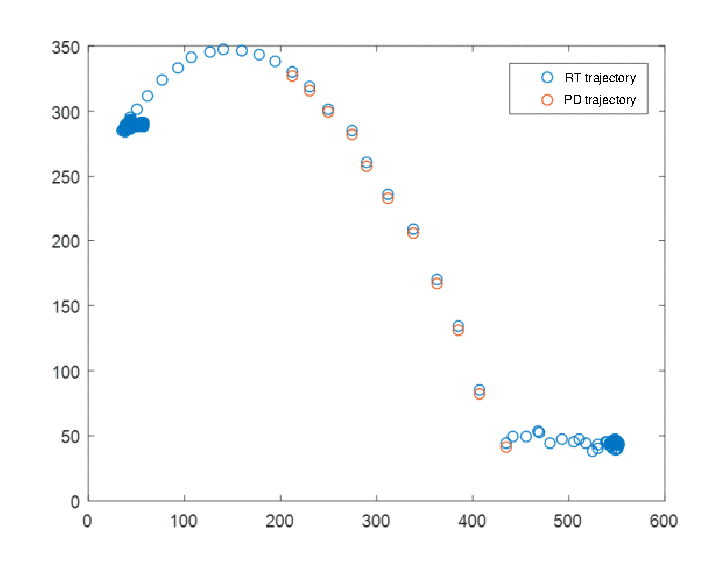
\includegraphics[width=3.5in]{fig/PFofRobot.pdf}
	\caption{ Trajectory captured by the cameras. The red point is the position where the ball is thrown, the blue points are the positions where to predict the catching points, and the yellow points are the predictive catch points.}
	\label{fig:Trajectory}
\end{figure}

\subsection{Result}
Through the analysis of two cases, the proposed $VCA$ based flexible structure provides a generic method to address the visual servo control problem in $ePLC$. Based on the $VCA$ protocol, the algorithms in $VS$ and $ES$ have a kind of normative correspondence and the existing modules and motion control algorithms could be reused without additional programing. 
\section{Conclusion}
\label{conclusion}
We propose a flexible multi-level architecture which is based on a $VCA$ protocol to integrate the PLC system, motion control system, and visual system to ease the complexity of the applications. The multi-level includes flexible layer, control layer, and algorithm layer. The $VCA$ protocol is designed for data interaction between the layers. Correspondingly, a customized hardware, memory allocation, Petri-Net based multithreading structure are described to support the proposed flexible software architecture. We implements two cases, the winding machine with visual system and the binocular catching robot, to illustrate the proposed system which provides a generic method to develop different type applications of visual servo system in $ePLC$.

In the further research, we will implement a uniform development method of the visual servo control in ePLC.

\ifCLASSOPTIONcaptionsoff
  \newpage
\fi



% trigger a \newpage just before the given reference
% number - used to balance the columns on the last page
% adjust value as needed - may need to be readjusted if
% the document is modified later
%\IEEEtriggeratref{8}
% The "triggered" command can be changed if desired:
%\IEEEtriggercmd{\enlargethispage{-5in}}

% references section

% can use a bibliography generated by BibTeX as a .bbl file
% BibTeX documentation can be easily obtained at:
% http://www.ctan.org/tex-archive/biblio/bibtex/contrib/doc/
% The IEEEtran BibTeX style support page is at:
% http://www.michaelshell.org/tex/ieeetran/bibtex/
%\bibliographystyle{IEEEtran}
% argument is your BibTeX string definitions and bibliography database(s)
%\bibliography{IEEEabrv,../bib/paper}
%
% <OR> manually copy in the resultant .bbl file
% set second argument of \begin to the number of references
% (used to reserve space for the reference number labels box)

\bibliographystyle{IEEEtran}
\bibliography{reference}

% biography section
%
% If you have an EPS/PDF photo (graphicx package needed) extra braces are
% needed around the contents of the optional argument to biography to prevent
% the LaTeX parser from getting confused when it sees the complicated
% \includegraphics command within an optional argument. (You could create
% your own custom macro containing the \includegraphics command to make things
% simpler here.)
%\begin{IEEEbiography}[{\includegraphics[width=1in,height=1.25in,clip,keepaspectratio]{mshell}}]{Michael Shell}
% or if you just want to reserve a space for a photo:

%\begin{IEEEbiography}[{\includegraphics[width=1in,height=1.25in,clip,keepaspectratio]{fig/Author_HuifengWu.eps}}]{Huifeng Wu} received the Ph.D. degree in computer science and technology from Zhejiang university, Hangzhou, China, in 2006. He is currently a professor in the institute of intelligent and software Technology, Hangzhou Dianzi University. His research interests include software development methods and tools, software architecture, embedded system, intelligent control \& automation.
%	
%\end{IEEEbiography}
%\begin{IEEEbiography}[{\includegraphics[width=1in,height=1.25in,clip,keepaspectratio]{fig/Author_YiYan.eps}}]{Yi Yan} received B.S. in automatic control engineering form Zhejiang Sci-Tech University in 1984, M.S. in computer engineering from Beijing University of Postal Telecommunications in 1990. Currently he is the director and full professor in institute of intelligent and software Technology, Hangzhou Dianzi University. His research interests include embedded system, advanced manufacturing system, intelligent control \& automation, and intelligent instruments.
%	
%	
%\end{IEEEbiography}
%\begin{IEEEbiography}[{\includegraphics[width=1in,height=1.25in,clip,keepaspectratio]{fig/Author_DanfengSun.eps}}]{Danfeng Sun} received M.S. in computer architecture from Hangzhou DianZi University in 2011. He is currently a research assistant in the Institute of Industrial Internet, Hangzhou DianZi University. His research interests include embeded system, motion control and IIoT.
%\end{IEEEbiography}
%\begin{IEEEbiography}[{\includegraphics[width=1in,height=1.25in,keepaspectratio,angle=-90]{fig/Author_ReneSimon.eps}}]{Rene Simon} obtained a doctor of engineering at the Otto-von-Guericke University Magdeburg in 2001. He is Professor of Control Systems at the Department of Automation and Computer Sciences, Harz University of Applied Sciences, Wernigerode, Germany. His major research fields include engineering of automation systems, especially industrial controllers. He is chairman of PLCopen and project leader IEC 61131-10 Ed. 1.0.
%\end{IEEEbiography}



% insert where needed to balance the two columns on the last page with
% biographies
%\newpage


% You can push biographies down or up by placing
% a \vfill before or after them. The appropriate
% use of \vfill depends on what kind of text is
% on the last page and whether or not the columns
% are being equalized.

%\vfill

% Can be used to pull up biographies so that the bottom of the last one
% is flush with the other column.
%\enlargethispage{-5in}



% that's all folks
\end{document}


